\chapter{Extracellular conductivity}
\label{chap:Sigma}
\index{Conductivity}
In \fref{chap:Neuron} we saw that neural activity causes transmembrane currents, and 
in \fref{chap:VC} we introduced volume conductor (VC) theory, a framework that links such transmembrane currents to extracellular potentials, based on some simple assumptions about how
currents move through the extracellular space.

In most applications of VC theory, the conductivity of brain tissue ($\sigma_\text{t}$) is assumed to be a constant, 
and its value is normally taken from some experimental measurement. 
Estimates of $\sigma_\text{t}$ vary between different recordings, 
but common values are between 0.3 and 0.5  \si{S/m} \cite**{Ranck1963,Logothesis2007,Goto2010,Elbohouty2013,Wagner2014,Miceli2017,McCann2019}.

\ghnote{Forsoekte aa oppsummere estimater av "typisk sigma" i en tabell, men det ble saa mye bal at jeg kommenterte den bort. 
Det ble krevende aa fordi maalingene generelt rapporterer masse greier og spesialtilfeller, noen er grey matter, noen er cortex, noen er brain, noen ser paa f-avhengighet, lagavhengighet, anisotropi etc. Og saa rapporteres det alltid en del ulike verdier i hvert paper - dvs. hvis vi skal skrive om det maa vi muligens gaa grundigere til verks og forklare eksperimentelle detaljer. Er det noe vi vil? Miceli-figuren som kommer lenger ned har jo gjort en del av dette arbeidet, og oppsummert eksperimenter som ser paa  f-avhengighet. Det finnes dog eksperimenter som ser paa andre ting.

Den angitte typiske range 0.3 -- 0.5 er ok nok, selv om de fleste av siteringene begynner paa 0.3 men ofte strekker seg utover dette. Unntaket er Goto som legger seg fast rundt 0.3. Saa finnes det jo dessuten saanne som Gabriel og greier samt noen eldre maalinge i ei bok av Y Fung, som ligger lavere enn 0.3. Vil vi gaa mer inn paa dette, eller rekker det med det som staar? Jeg har brukt 0.3 som en typisk verdi i noen regneeksempler under. Boer den byttes, eller er 0.3 ok?

Hvis vi (dere) har brukt en standardverdi for sigma i deres simuleringer saa kan dette vaere et ok sted aa oppgi den paa.
}
%\begin{table}[h!]
%\begin{center}
%\caption[Tissue conductivity]{$\sigma_\text{t}$ (\si{S/m}) estimates from various sources in the frequency range up to 10 kHz.}
%\label{tab:Sigma:diffconsts}
%    \begin{tabular}{l|l}
%    \hline
%    $Grey matter$ & 0.03--0.4$ \, \si{S/m} & \cite**{Martinsen2008}\\ \hline
%    $Grey matter$ & $0.47 \pm 0.24$\, \si{S/m} & \cite**{McCann2019} \\ \hline
%    $Cortex$ & 0.03 --0.1 \, \si{S/m} $ \cite**{Gabriel1996}\\ \hline 
%    $Cortex$ & 0.3 --0.6 \, \si{S/m} $ \cite**{Wagner2014}\\ \hline 
%    $Cortex$ & 0.3 --0.4 \, \si{S/m} $ \cite**{Elbohouty2013}\\ \hline 
%    $Cortex$ & 0.4 -- 0.6 \, \si{S/m} $ \cite**{Miceli2017}\\ \hline 
%    $Cortex$ & 0.3 -- 0.4 \, \si{S/m} $ \cite**{Ranck1963}\\ \hline 
%    $Cortex$ & 0.4 -- 0.5 \, \si{S/m} $ \cite**{Logothesis2007}\\ \hline 
%    \end{tabular}
%\end{center}
%\end{table}

%\ghtxt{Hva er en bra range aa oppgi her? Micelifiguren oppsummerer studier som har sett paa f-avhengighet, men det finnes i tillegg mange maalinger som ikke har den ambisjonen. I Oerjanboka staar det at $\sigma$ for grey matter er 0.03 -- 0.4 S/m i omraadet 1 Hz til 10 kHz. Nunez sier 0.29 \,\si{S/m} for cortex, 5 Hz. McCann 2019 oppsummerer et sammensurium av ulike maaleteknikker som gir ganske ulike resultater, men lander en slags konklusjon om $0.47 \pm 0.24 \,\si{S/m}$ (grey matter), som da lander paa mye hoeyere verdier enn Oerjan Martinsens 0.03 -- 0.4 \si{S/m}  (grey matter). Miceli ligger ml. 0.03 og 0.7. Grodzinsky har en tabell der de angir verdier paa 1 kHz, og en range  0.13 (kanin) -- 0.22 (misc) \, \si{S/m}. Okada 1994 sa at skillpaddecerebellum laa paa 0.15 (molecular layer) -- 0.25 (granular layer). Er dette noe vi skal skrive om? Goto 2010 sier 0.3 S/m grey matter/cortex.}

%$\sigma_\text{greymatter}$ range from 0.03 -- 0.4 \si{S/m} in grey matter \cite**{Martinsen2008}
%$\sigma_\text{greymatter} = 0.47 \pm 0.24 \, \si{S/m}$ \cite**{mccann2019}
%$\sigma_\text{whitematter} = 0.22 \pm 0.17 \, \si{S/m}$ \cite**{mccann2019}
%$\sigma_\text{t}$ ranges from 0.03 to 0.7 \si{S/m} \cite**{Miceli2017}
%$\sigma_\text{brain}$ range from = 0.13 (rabbit) -- 0.22 (misc) \, \si{S/m}, but there at 1 kHz \cite**{Grodzinsky2011}. 
%$\sigma_\text{t}$ range from = 0.15 (molecular layer) -- 0.25 (granular layer) \, \si{S/m} in turtle cerebellum 
%\cite**{Okada1994}. 

Throughout \Fref{chap:VC}, we assumed that $\sigma_\text{t}$ was constant, 
which amounts to assuming that brain tissue is \tvntxt{infinite, }homogeneous, isotropic and frequency independent.
\tvntxt{While these assumptions are in many cases appropriate, there are
also many cases where they are not appropriate, and}
in this chapter we discuss these assumptions and ways to relax them\tvntxt{\sout{, since neither of them are strictly true}}\tvnnote{Syntes dette ga inntrykk av at man alltid har lyst til aa bli kvitt disse forenklingene, men det er jo ikke tilfellet.}.
In addition, we review some experimental and theoretical estimates of $\sigma_\text{t}$. 

Before we start examining the properties of $\sigma_\text{t}$, we must establish a clear picture
of what it represents, i.e., what $\sigma_\text{t}$ is the conductivity \textit{of}.
Such a picture is established through the continuous, porous medium approximation that we introduce below. 


%%%%%%%%%%%%%%%%%%%%%%%%%%%%%%%%
\section{\blue{Continuous, porous medium approximation}}
\label{sec:Sigma:continuous}
\index{Continuous medium}\index{Porous medium}
%%%%%%%%%%%%%%%%%%%%%%%%%%%%%%%%
The idea of the brain as being composed of individual neurons communicating through synapses 
dates back to the works by Santiago Ram\'{o}n y Cajal in the late 19th century.
Using a silver-staining technique developed earlier by Camillo Golgi, 
Cajal was able to observe individual neurons in thin slices of brain tissue through a microscope, 
and illustrated them in his famous and beautiful drawings \cite**{cajal1899}.

\begin{figure}[!ht]
\begin{center}
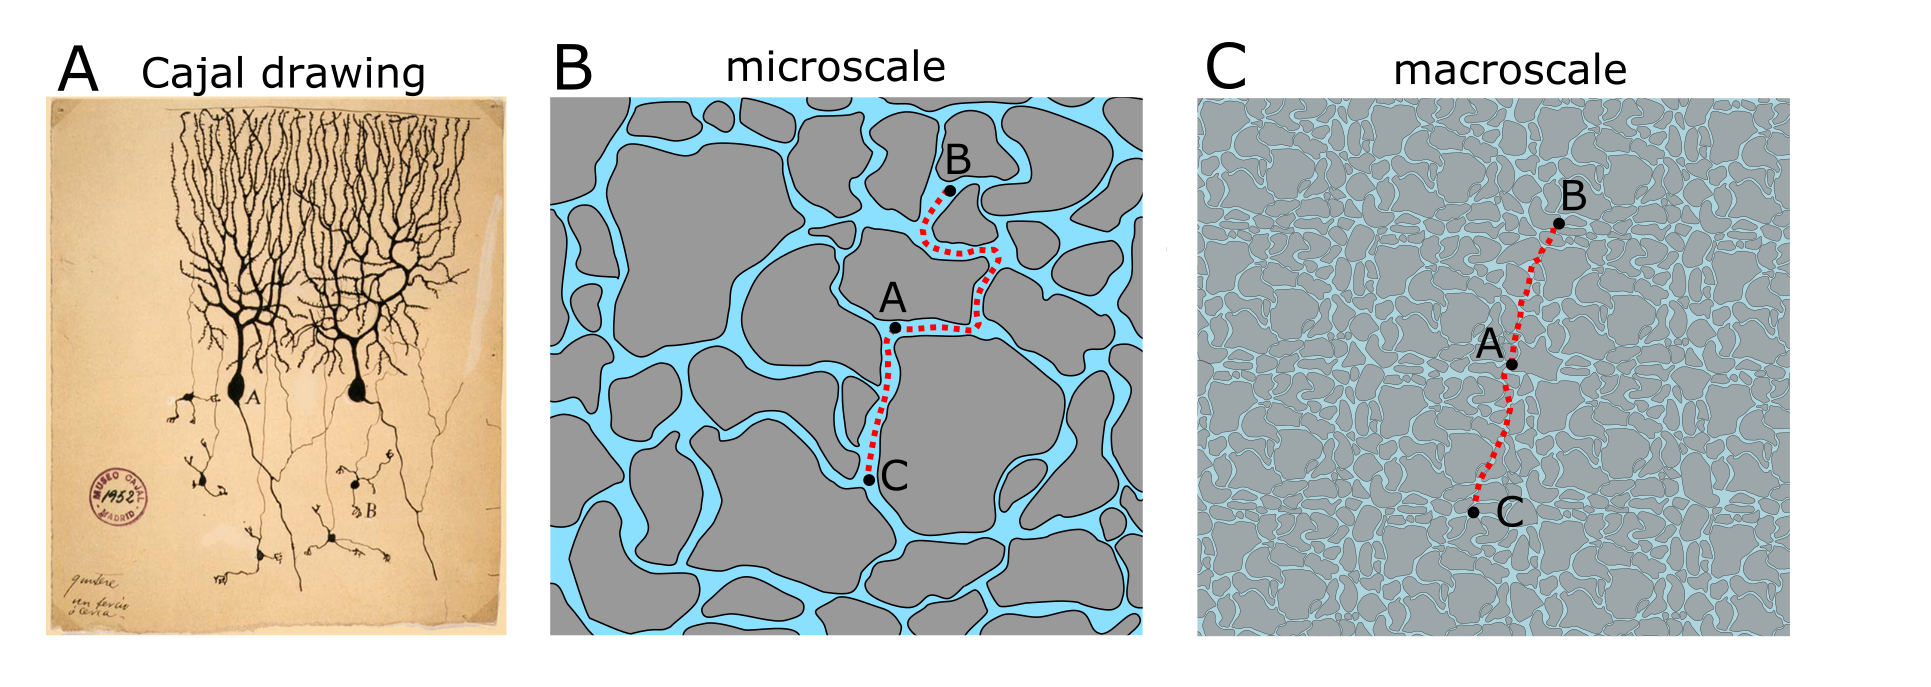
\includegraphics[width=0.9\textwidth]{Figures/Sigma/ecs2.png}
\end{center}
\caption[]{\textbf{Illustration of brain tissue.} 
({\bf A})  Example of Cajal drawing, depicting of purkinje neurons (downloaded from \url{https://commons.wikimedia.org}). 
({\bf B}) Illustration of a tissue transection. Extracellular space (light blue) occupies only a fraction $\alpha$ 
of the total tissue volume, and has a highly tortuous structure. The tortuosity, $\lambda$, 
is defined as the ratio between the shortest pathway between two points in space 
and the euclidian distance between these two points, 
and accounts for the fact that ions traveling through the medium do not travel in straight lines, 
but need to take detours around cellular obstacles. 
$\alpha$ and $\lambda$ vary on the microscopic scale. 
For example, the shortest path (red dotted curve) between locations $r_0$ and $r_1$ 
is more tortuous than the path between locations $r_0$ and $r_2$.  
({\bf C}) On a larger spatial scale, local inhomogeneities average out, 
and the tissue can be treated as homogeneous. 
Typical tissue averages for $\alpha$ and $\lambda$ are 0.2 and 1.6, respectively \cite**{Nicholson1998,Sykova2008}. 
\ghnote{La til en liten Cajal her. Ble saa mye figurer om den fikk staa aleine. Bildet er saa gammelt at det ikke blir opphavsrettproblemer,}}
\label{fig:Sigma:ECS}
\end{figure}

Judging from Cajal's drawings (an example is shown in \fref{fig:Sigma:ECS}A), 
brain tissue appears to be rather sparsely populated, with quite a lot of space between individual cells. 
Had this been the case, the tissue conductivity would have been close to that of the extracellular fluid. 
However, in experimental methods used by Cajal, only a small fraction of the neurons 
were actually stained and observed. In reality, the brain is so densely packed with neurons and glial cells 
that if they all had been stained, Cajal's images would have been pure black. 

As illustrated in \fref{fig:Sigma:ECS}B, the extracellular space (colored light blue in the figure) 
occupies only about 20\% of the total tissue volume, and has a highly tortuous \index{Tortuosity} geometry, 
with an average extracellular distance between cell membranes of only about 40-60~nm \cite**{Sykova2008}.
Currents passing through tissue are typically assumed to move predominantly through the extracellular space,
while the cell bodies largely act as non-conducting obstacles \cite**{Robinson1968,Nunez2006}. 
Tissue currents are then restricted to follow narrow winding paths 
through the small extracellular fraction of the tissue volume,
and we therefore expect the effective tissue conductivity to be lower than 
that of an obstacle-free saline solution. 

%\ghnote{Torbjorn foreslo:} \ghtxt{"From this, we can already make a first rough estimate of the extracellular conductivity: The extracellular saline solution has a conductivity of about 1.5~\si{\siemens\per\metre}, but only occupies about 20\% of the space, meaning that we might expect the extracellular conductivity to be on the order of 1.5~\si{\siemens\per\metre} $\cdot$ 0.2 = 0.3~\si{\siemens\per\metre}. This value fits well with the values typically measured in experiments, although the calculation itself vastly underestimates the complex electrical properties of neural tissue. "} \ghnote{Ganske fint, men tar ikke hensyn til tortuositeten, noe jeg gjoer i punktlisten ikke langt nedenfor her. Frykter derfor at dette grovestimatet vil forvirre leseren, naar et anelsen mindre grovt estimat foelger saa tett nedenfor.}

On a small spatial scale, the conductivity in a certain spatial direction 
will depend on whether there locally is a free extracellular passage in that direction (high conductivity), 
or whether this passage is blocked by a nearby membrane (low conductivity) (\fref{fig:Sigma:ECS}{\bf A}). 
At the spatial scale of micrometers and below, the extracellular conductivity\index{Conductivity} 
is therefore highly inhomogeneous and anisotropic. 

%Likewise, also the electric potential $\phi$ will vary greatly over tiny distances, depending on the proximity to neural membranes, especially when approaching the nanometer thick Debye-layers building up the membrane charge \cite**{Pods2013}\tvnnote{Kanskje denne setningen hoerer mer hjemme i VC eller Basics?}.
%When we study extracellular potentials, we are typically not interested in these microscopic variations in $\sigma$ and $\phi$, but rather in the values of these entities when averaged over some spatial volume. Electrodes used to record extracellular potentials typically have sizes ranging from 5 $\mu$m to 125 $\mu$m in diameter \cite**{Viswam2019}, which is larger than the typical diameter of a dendrite ($\sim$ 1 $\mu$m). In practice, the electrodes therefore perform such an averaging, and include contributions from several nearby neurons \tvnnote{Remove last half of sentence? Seems like a different issue to me}. \tvnnote{Tok bort dette, da jeg tenker vi dekker dette et annet sted?}
At a larger spatial scale of, say, hundreds of micrometers, 
it is reasonable to assume that the micrometer scale inhomogeneities average out (\fref{fig:Sigma:ECS}{\bf B}), 
so that brain tissue can be treated as a continuous, porous medium \cite**{Nicholson1981,Nicholson2001,Gratiy2017}. 
Such a treatment is further motivated by the lack of any alternative way to approach the problem, 
since we in most experimental settings do not know the exact microstructure of the brain. 
The VC theory presented in the previous chapter was based on the continuous, porous medium approximation, 
and thus describes the extracellular dynamics on a coarse-grained spatial resolution ($\gg 1 \si{\micro\metre}$)
as defined in \fref{sec:Basics:ECSpot}.

A continuous, porous medium is defined by two key parameters \cite**{Nicholson1981}. 
The first parameter, $\alpha$, is the fraction of the tissue volume that is extracellular space. 
The second parameter, $\lambda$, is the tortuousity of the extracellular medium, 
defined as the ratio between the shortest extracellular pathway between two points in space 
and the euclidian distance between these two points. 
The tortuousity accounts for the fact that ions traveling through the medium do not travel in straight lines, 
but need to take detours around cellular obstacles. 
The parameters $\alpha$ and $\lambda$ can be measured experimentally. 
Typical values are $\alpha = 0.2$ and $\lambda = 1.6$ \cite**{Sykova2008}, 
although these values can vary quite substantially between brain regions, 
and also locally with in a brain region, due to brain-state dependent cellular swelling or shrinkage \cite**{Sykova2008,rasmussen2020}.

The continuous, porous medium approximation has implications 
for how we interpret the various concepts and variables that we use to compute extracellular potentials. 
In particular, it is important for how we understand the conductivity of the tissue medium. 
Below, we give an interpretation of what the tissue conductivity ($\sigma_\text{t}$) represents. 
To do this, we first define two additional conductivity measures: 
(i) that of the extracellular saline solution ($\sigma_\text{saline}$), and 
(ii) that of the extracellular medium ($\sigma_\text{e}$), and then explain how 
(iii) the tissue conductivity ($\sigma_\text{t}$) relates to those. 


\subsection{\blue{Conductivity of saline: $\sigma_\text{saline}$}}
\label{sec:Sigma:Ssaline}
\index{Conductivity! of saline solution}
$\sigma_\text{saline}$ (\si{S/m}) is the conductivity of the saline solution that fills up the extracellular space. 
$\sigma_\text{saline}$ defines the (very) local conductivity within the small gaps between cellular bodies,
and is not the conductivity of brain tissue as a whole. 

The conductivity generally depends on the availability of free charge carriers, 
and $\sigma_\text{saline}$ is therefore determined by the ion concentrations in the saline solution:
\begin{equation}
\sigma_\text{saline} = \frac{F^2}{RT}\sum_{k} D_k z_{k}^2 c_{k}.
\label{eq:Sigma:sigma1}
\end{equation}
We have previously shown how this definition of the conductivity follows from the Nernst-Planck equation (see \fref{eq:Basics:sigma_conc}). We recall that $z_{k}$, $D_k$ and $c_{k}$ denote the valency, diffusion coefficient and concentration, respectively, of ion species $k$, while $F = 96485.3 \, \si{C/mol}$ is the Faraday constant, 
$R = 8.314 \,\si{J/(K \, mol)}$ is the gas constant, and $T$ (\si{\kelvin}) the temperature.

Typical concentrations of the most abundant ions in the extracellular saline solution were listed in 
\fref{tab:Neuron:ion-concentrations}, and their diffusion constants are given in \fref{tab:Sigma:diffconsts}. 
If we insert the values from \fref{tab:Neuron:ion-concentrations} and \fref{tab:Sigma:diffconsts} into \fref{eq:Sigma:sigma1}, 
and assume a body temperature of $T = 310\, \si{\kelvin}$, 
we get a conductivity $\sigma_\text{saline} = 1.72 \, \si{S/m}$. 

\begin{table}[h!]
\begin{center}
\caption[Diffusion Constants]{Diffusion constants for ions in dilute solutions. Values taken from from \cite**{Bowen2002,Lyshevski2007}}
\label{tab:Sigma:diffconsts}
    \begin{tabular}{l|l}
    \hline
    $D_\text{Na}$ & $1.33\times 10^{-9}$ \, \si{m^2/s}\\ \hline
    $D_\text{K}$ & $1.96  \times 10^{-9}$ \, \si{m^2/s} \\ \hline
    $D_\text{Cl}$ & $2.03 \times 10^{-9}$ \, \si{m^2/s} \\ \hline
    $D_\text{Ca}$ & $0.71\times 10^{-9}$ \, \si{m^2/s}\\ \hline
    $D_\text{Mg}$ & $0.72\times 10^{-9}$\, \si{m^2/s} \\ \hline
    $D_\text{HCO3}$ & $1.18\times 10^{-9}$ \, \si{m^2/s} \\ \hline
    \end{tabular}
\end{center}
\end{table}

Note that the extracellular solution contains many ion species (such as e.g., H$^+$ and HPO4$^{2-}$ ) 
that were not included in Table \ref{tab:Neuron:ion-concentrations}, and thus not in our calculation of $\sigma_\text{saline}$. 
However, concentrations of ions others than those in Table \ref{tab:Neuron:ion-concentrations} are generally quite low, 
and therefore not likely to have any major impact on the conductivity. Note also that the the extracellular concentrations 
listed in \fref{tab:Neuron:ion-concentrations} were based on reported values in the human cerebrospinal fluid, 
and that saline concentrations may deviate from this in other tissues. 
Our estimated value of $\sigma_\text{saline}$ nevertheless seems to be quite representative,
and agrees well with experimentally reported values of $\sigma_\text{saline}$, 
which typically range between 1.3 and 1.8~\si{S/m}\cite**{Okada1994,Baumann1997,Logothetis2007,Martinsen2008,Miceli2017,mccann2019}.



\subsection{\blue{Conductivity of extracellular space: $\sigma_\text{e}$}}
\label{sec:Sigma:Se}
$\sigma_\text{e}$ (\si{S/m}) is the conductivity of the \textit{extracellular medium}\index{Extracellular medium}. 
As we define it here, it is a theoretical quantity, 
representing the conductivity experienced by a \textit{hypothetical} macroscopic (coarse-grained) current 
that travels exclusively trough the extracellular part of brain tissue. 
This current does not pass through a 3D volume filled entirely by extracellular saline, 
but is (i) restricted to move only through the fraction $\alpha$ of the total medium volume that is extracellular, 
and (ii) must take detours around neural and glial obstacles, 
as reflected through the tortuousity $\lambda$ \cite**{Nicholson1998,Nunez2006}. 

If we account for the extracellular volume fraction and tortuous structure of the extracellular space, 
the extracellular conductivity should theoretically be a factor $\alpha/\lambda^2$ lower than saline conductivity \cite**{Okada1994}:

\begin{equation}
\sigma_\text{e} = \frac{\alpha}{\lambda^2} \sigma_\text{saline}.
\label{eq:Sigma:sigmat}
\end{equation}
Typical values for $\alpha$ and $\lambda$ for the extracellular space of brain tissue 
are 0.2 and 1.6, respectively \cite**{Nicholson1981,Nicholson1998,Sykova2008}. 
With these values, $\sigma_\text{e}$ becomes almost a factor 13 lower than $\sigma_\text{saline}$, 
and with the above estimate, $\sigma_\text{saline} = 1.72 \, \si{S/m}$, 
we get a an estimated value $\sigma_\text{e} = 0.134\, \si{S/m}$. 




\subsection{\blue{Conductivity of brain tissue: $\sigma_\text{t}$}}
\label{sec:Sigma:St}
$\sigma_\text{t}$ (\si{\siemens\per\metre}) is the macroscopic (coarse-grained) conductivity of the brain tissue, 
i.e., the conductivity experienced by a macroscopic (coarse-grained) current traveling through the tissue. 
It is $\sigma_\text{t}$ that one normally measures experimentally, 
and it is $\sigma_\text{t}$ that is the relevant conductivity for use in VC theory. 

If currents through brain tissue were indeed confined to stay exclusively in the extracellular part of it, 
$\sigma_\text{t}$ should be identical to $\sigma_\text{e}$, defined above. 
However, if tissue currents to some degree cross membranes and take intracellular pathways 
in addition to the extracellular ones, we would expect $\sigma_\text{t}$ to be greater than $\sigma_\text{e}$.

Measured values of $\sigma_\text{t}$ vary quite much between different experiments, 
but a typical value is $\geq 0.2 \, \si{\siemens\per\metre}$, 
which is higher than the value $\sigma_\text{e} = 0.134\, \si{\siemens\per\metre}$ that we estimated above. 
The reason why the estimated $\sigma_\text{e}$ is lower than $\sigma_\text{t}$, 
is expectedly that a fraction of the real tissue currents do travel through intracellular pathways. 
For example, in experiments done in the turtle cerebellum, 
it was estimated that about 50 \% of tissue currents travel through intracellular paths \cite**{Okada1994}. 

\ghnote{Muligens putte inn noe Meffin-greier her.}


\section{\blue{Frequency dependence of the tissue conductivity}}
\label{sec:Sigma:f-independent}
\index{Conductivity!Frequency dependence}
%\ghnote{GH: Skrev skisse til dette. Puttet figuren m/ sigma-maalinger inn her, da disse ser ut til aa primaert diskuteres opp mot eventuell frekvensavhengighet. Mulig vi burde ha med "eksperimentelle maalinger i kapittel-tittelen?}
%Regardless of the level of isotropy and homogeneity of a medium, its response to an imposed alternating current can depend on the frequency of the current. Then, the conductivity contains a resistive part, which is real and frequency independent, and an imaginary part that accounts for capacitive and inductive effects that are frequency dependent.
An important question when modeling and interpreting electric signals in neuroscience 
is whether the conductivity of neural tissue ($\sigma_\text{t}$) has a frequency dependence 
(also called the impedance spectrum). 
If it does, recorded signals will be distorted as they propagate through the tissue, 
which in turn will bias recordings towards certain parts of the frequency spectrum. 
In this subsection we will briefly review some experimental measurements investigating this issue, 
as well as the theory needed to model such effects, should it be deemed necessary.

As we stated earlier, 
extracellular currents often are assumed to move mostly through the extracellular saline solution
between cells that constitute passive, non-conducting obstacles (\fref{sec:Sigma:continuous}). 
If this is true, we would expect $\sigma_\text{t}$ to be frequency-independent,
since saline is known to be a purely resistive medium, at least up to frequencies in the megahertz range
\cite**{cooper1946,Martinsen2008}.

A frequency dependent $\sigma_\text{t}$ would, however, not in itself be surprising.
Capacitive neural membranes have a highly frequency dependent conductivity (\fref{sec:Neuron:Cap}),
and one could easily imagine that low-frequency tissue currents are prone to pass resistively through the extracellular space, 
while high-frequency tissue currents pass both resistively through the extracellular space and capacitively through cells. 
This would effectively cause $\sigma_\text{t}$ to increase with frequency and, as a consequence, 
the amplitude of extracellular potentials to decrease with frequency (see \fref{eq:Sigma:pointsource_freq_dep}). 
If such effects were present, we would for example expect the low-frequency LFP signals 
to be less attenuated with distance compared to high-frequency spikes. 
Such a frequency bias has been suggested as the explanation behind ...
It has been suggested that "stability" of LFP and sensitivity of spikes to position is caused 
by this, and EEG has "only" low frequencies \cite**{Logothetis2007}, and 1/f power-laws in LFP \tvnnote{Expand a little on this and cite the French}. \ghnote{Forsto ikke helt setningen, men antar, som du antyder, at den er uferdig.}

Early investigations indicated that $\sigma_\text{t}$ has little or no frequency dependence \cite**{Ranck1963,nicholson1975,Pfurtscheller1975}.
This was later challenged by \citeasnoun**{Gabriel1996}, who measured
a substantial frequency dependence of $\sigma_\text{t}$, in particular below 100~\si{\hertz} (\fref{fig:Sigma:freq_dep}). 
A series of more recent studies again seemed to reconfirm the early finings, 
and measured a $\sigma_\text{t}$ that did not depend or depended very little on stimulus frequency \cite**{Logothetis2007,Elbohouty2013,Wagner2014,Dowrick2015,Miceli2017,Ranta2017,Avery2017}. 
Notably, many of these recent studies consistently measured a moderate increase of $\sigma_\text{t}$ 
by about 20-50\% when the stimulus frequency was increased from a few hertz to some hundreds or thousands of hertz (\fref{fig:fig:Sigma:freq_dep}), but two of them also measured a similar frequency dependence in (pure) saline, 
indicating that this frequency dependence at least partially originated in the recording equipment \cite**{Logothetis2007,Miceli2017}. 

\begin{figure}[!ht]
\begin{center}
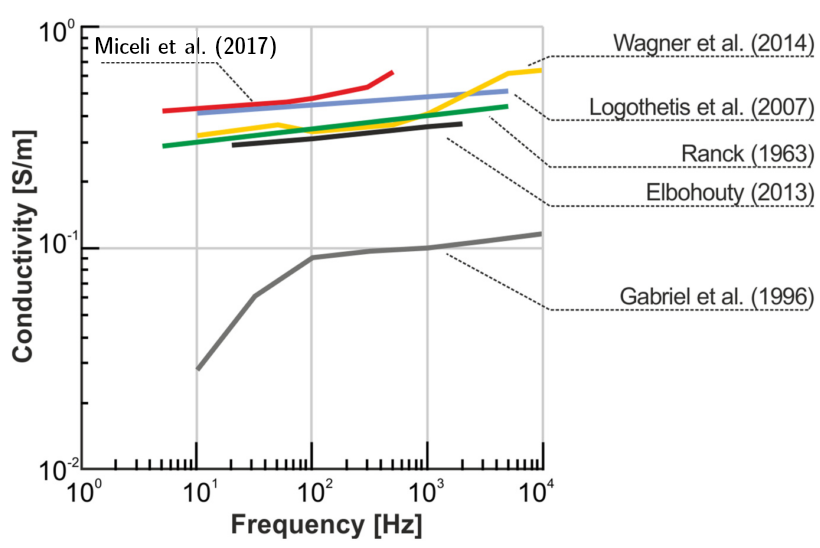
\includegraphics[width=0.6\textwidth]{Figures/Sigma/frequency_dependence.png}
\end{center}
\caption[]{\textbf{Literature review of reported conductivities in various species and experimental setups.}
Most studies seem to indicate a very weak frequency dependence of the tissue conductivity\index{Conductivity}, 
which would have a negligible effect on measured extracellular potentials \cite**{Miceli2017}. 
The very low and strongly frequency dependent values measured by \cite**{Gabriel1996} represents an outlier, 
and although it has received substantial attention, it has to the best of our knowledge not been reproduced by any other study. For details about the data, see \cite**{Miceli2017}, and references therein \cite**{Ranck1963,Gabriel1996,Logothetis2007,Elbohouty2013,Wagner2014}.
}
\label{fig:Sigma:freq_dep}
\end{figure}

To our knowledge, the study by \citeasnoun**{Gabriel1996} is the only experimental study 
to find a strong frequency dependence for low frequencies. 
This study also stands out in that it reported a conductivity of only about 0.03~\si{\siemens/ \metre} at 10~\si{\hertz}, 
about an order of magnitude lower than the commonly reported values. 
This value seems surprisingly low, given that healthy neural tissue contains a substantial fraction of highly conducting saline. 
The authors were however careful to note that the reported low-frequency values might be distorted 
by inadequate correction for electrode polarization (see \fref{sec:VC:electrodes} for a brief review of electrode polarization). 
In addition, their recording were done in bovine brains obtained from a slaughterhouse 
up to a couple of hours post-mortem \cite**{Gabriel1996}, 
which can potentially have resulted in suboptimal tissue preservation and cell swelling. 
Finally, we note that a later study using the same recording equipment did not observe a similarly strong frequency-dependence, 
or similarly low conductivity values (\citeasnoun**{Wagner2014}; \fref{fig:Sigma:freq_dep}). 

Consequently, experimental evidence suggests that neural tissue is predominantly resistive, 
having at most a weak frequency dependency of the order of up to $\sim$30\% 
over the frequency range of interest for neurophysiology (below a few thousand hertz). 
This might not sound very small, but modeling studies have indicated 
that frequency dependencies of this order would have a relatively minor effect 
on measured potentials of physiological origin \cite**{Bossetti2008,Tracey2011,Miceli2017}
\tvnnote{Add figure adapted from Miceli2017?}. 
We note however that this is not necessarily true for potentials evoked by extracellular current stimulation 
using very brief current pulses, because of the very high frequency content of the pulses \cite**{Bossetti2008}.
 \ghtxt{We will revisit the topic of electrode stimulations in \fref{chap:Stim}, but will for now focus on physiological signals.}

%\subsection{\red{Complex conductivity}}
%\label{sec:Sigma:Complex}
%If capacitive effects are present in tissue currents, 
%these can be accounted for is the CSD equation (\fref{eq:Basics:continuity2}) 
%by replacing the tissue conductivity $\sigma_\text{t}$ with a complex conductivity $\sigma_\text{c}$:
%\begin{equation}
%{\bf \nabla} \cdot \left(\sigma_\text{c} {\bf \nabla} {\phi} \right) = -C,
%\label{eq:Sigma:compexCSD}
%\end{equation}
%where $\sigma_\text{c} = \sigma_\text{c}(\omega)$ depends on the the angular frequency $\omega = 2 \pi f$ of the electric field. 
%
%To define this complex conductivity, we start with the total (conductive plus capacitive) current through the medium:
%\begin{equation}
%{\bf i} = \sigma_\text{t}{\bf E} +  \epsilon \frac{\partial {\bf E}}{\partial t},
%\label{eq:Sigma:itot}
%\end{equation}.
%and consider an oscillatory electric field:
%\begin{equation}
%{\bf E} = {\bf E}_{max}e^{j\omega t}, 
%\label{eq:Sigma:Eomega}
%\end{equation}.
%where $j$ is the imaginary unit, and $\omega$ the angular oscillation frequency of field (or a component of it). If we insert \fref{eq:Sigma:Eomega} into \fref{eq:Sigma:itot}, we can write the current as:
%\begin{equation}
%{\bf i} = \left( \sigma_\text{t} + j\omega \epsilon \right) {\bf E}, 
%\label{eq:Sigma:itot2}
%\end{equation}
%or as:
%\begin{equation}
%{\bf i} = \sigma_\text{c} {\bf E}, 
%\label{eq:Sigma:itot3}
%\end{equation}
%where we have introduced the complex conductivity:
%\begin{equation}
%\sigma_\text{c} = \sigma_\text{t}(\omega)\left(1 + \frac{j \omega \epsilon(\omega)}{\sigma_\text{t}(\omega)} \right).
%\label{eq:Sigma:complex}
%\end{equation}
%We note that \fref{eq:Sigma:itot3} is generally only valid in the frequency domain, while in the time domain, ${\bf i}$ must be given as a temporal convolution of $\sigma$ and ${\bf E}$ \cite**{Bedard2009}. \ghnote{Jeg tok dette fra Pettersen 2012. Skal vi si mer om saken, eller holder dette? Vi har ikke forklart hva time-domain og frequency-domain betyr.}
%
%The real and imaginary parts of $\sigma_\text{c}$ correspond to the conductive and capacitive properties of the medium, respectively. As indicated, both components can have an individual frequency dependence through $\sigma_\text{t}(\omega)$ and $\epsilon(\omega)$. \ghnote{Burde nok si noe om hvorfor $\sigma_t$ "plutselig" er frekvensavheng "internt" - det kunne den vel ogsaa ha vaert tidligere, dvs. uten at vi hadde med kapasitivt ledd?} However, we note that these "individual" frequency dependencies are not independent: To obey causality, that is, that the extracellular potential originating from a current can not precede the current, there must be a certain relationship between $\sigma_\text{t}(\omega)$ and $\epsilon(\omega)$, which can be found from the Kramers-Kronig relation, or equivalently from the Bode relation between the magnitude of the conductivity $|\sigma(\omega)|$ and the induced phase-shift $\exp ^{-{\bf j} \theta(f)}$. \ghnote{Det stemmer sikkert, men foeler det trengs noe mer her. I det minste noen referanser?}
%
%If we use \fref{eq:Sigma:compexCSD} with a complex conductivity as a starting point for VC theory,  the point-source equation (\fref{eq:VC:pointsource}) becomes \cite**{plonsey1967,Bossetti2008,Miceli2017}:
%\begin{equation}
%\phi({\bf r}, \omega) = \frac{I(\omega)}{4\pi (\sigma_\text{t}(\omega) + j \omega \epsilon(\omega)) r},
%\label{eq:Sigma:pointsource_freq_dep}
%\end{equation}
%\tvnnote{notation must be fixed. }
%\ghnote{fixed it. I kept the imaginary unit in math-mode - i think this is the standard?}
%
%
%

\subsection{\blue{Complex conductivity}}
\label{sec:Sigma:Complex}
\ghnote{Tidligere brukte vi $\sigma_\text{c}$ for kompleks konduktivitet, 
og lot da $\sigma_\text{t}$ vaere realdelen av denne. 
I ny versjon har jeg latt $\sigma_\text{t}$ ALLTID vaere tissue-konduktiviteten,
enten den er frekevsavhengig eller ei. Ok?}

%\begin{equation}
%\sigma_\text{t} = \sigma_\text{r} + j\sigma_\text{c}
%\label{eq:Sigma:ComplexSigma}
%\end{equation}
%where $j$ is the imaginary unit, and where $\sigma_\text{Re}$ and $\sigma_\text{Im}$
%are real and imaginary parts of
If (linear) capacitive effects are present in tissue, 
they can be incorporated into the theory by allowing the tissue conductivity to be complex
and frequency dependent.

To define this complex conductivity, we start with the total (resistive plus capacitive) 
current density through the medium:
\begin{equation}
{\bf i} = \sigma_\text{R}{\bf E} +  \epsilon \frac{\partial {\bf E}}{\partial t},
\label{eq:Sigma:itot}
\end{equation}
where we have let $\sigma_\text{R}$ denote the real (purely resistive) part of the tissue conductivity.
We seek to write this on the linear form:
\label{eq:Sigma:itot}
\begin{equation}
{\bf i} = \sigma_\text{t}(\omega) {\bf E},
\label{eq:Sigma:itot3}
\end{equation}
where $\sigma_\text{t}(\omega)$ is identical to $\sigma_\text{R}$ only in the case
when the medium is purely resistive. 

Next, we consider an oscillatory electric field:
\begin{equation}
{\bf E} = {\bf E}_{max}e^{\mathrm{j}\omega t}, 
\label{eq:Sigma:Eomega}
\end{equation}
where $\mathrm{j}$ is the imaginary unit, and $\omega$ the angular oscillation frequency of field (or a component of it). 
If we insert \fref{eq:Sigma:Eomega} into \fref{eq:Sigma:itot}, we can write the current density as:
\begin{equation}
{\bf i} = \left( \sigma_\text{R} + \mathrm{j}\omega \epsilon \right) {\bf E}.
\label{eq:Sigma:itot2}
\end{equation}
Further, we realize that we can write this on the linear form in \fref{eq:Sigma:itot3}
if the complex conductivity defined by:

\begin{equation}
\sigma_\text{t}(\omega) = \sigma_\text{R}\left(1 + \frac{\mathrm{j} \omega \epsilon}{\sigma_\text{R}} \right).
\label{eq:Sigma:complex}
\end{equation}

The real and imaginary parts of $\sigma_\text{t}(\omega)$ correspond to the 
resistive and capacitive properties of the medium, respectively. 
If we use a complex conductivity as a starting point for VC theory,  
the point-source equation (\fref{eq:VC:pointsource}) becomes \cite**{plonsey1967,Bossetti2008,Miceli2017}:
\begin{equation}
V_\mathrm{e}({\bf r}, \omega) = \frac{I(\omega)}{4\pi (\sigma_\text{R}) + \mathrm{j} \omega \epsilon) r},
\label{eq:Sigma:pointsource_freq_dep}
\end{equation}

\ghnote{Flyttet all problematisering til slutten:}
We note that \fref{eq:Sigma:itot3} is generally only valid in the frequency domain, 
while in the time domain, ${\bf i}$ must be given as a temporal convolution 
of $\sigma_\mathrm{t}$ and ${\bf E}$ \cite**{Bedard2009}. Only in the case when 
the $\sigma_\mathrm{t}$ is frequency independent, it is valid also in the time domain. 
\ghnote{Skal vi si mer om saken, eller holder dette? Vi har ikke forklart hva time-domain og frequency-domain betyr.}

We also note that we in the above focused on the frequency dependence due to capacitive properties in the medium.
In addition to this, the real part of the conductivity and the permittivity may have "individual" frequency dependencies, 
so that $\sigma_\text{R}=\sigma_\text{R}(\omega)$ and $\epsilon = \epsilon(\omega)$, 
thus causing the real and imaginary components of \fref{eq:Sigma:pointsource_freq_dep} 
to have individual frequency dependencies.
Importantly, these "individual" frequency dependencies are not independent: 
To obey causality, that is, that the extracellular potential originating from a current can not precede the current, 
meaning that there must be a certain relationship between $\sigma_\text{R}(\omega)$ and $\epsilon(\omega)$.
This relationship can be found from the so-called \textit{Kramers-Kronig relation}, 
or equivalently from the \textit{Bode relation} between the magnitude of the conductivity 
$|\sigma_\text{R}(\omega)|$ and the induced phase-shift $\exp ^{-{\bf j} \theta(f)}$ \cite**{Miceli2017}. 
\ghnote{Det stemmer sikkert, men foeler det trengs noe mer her. I det minste noen referanser? La til ref til Miceli, der det staar noe om Bode. Andre refs?}

\ghnote{Burde vi si mer om hvorfor $\sigma_R$ "plutselig" ble frekvensavheng akkurat her? 
Det kunne den vel ogsaa ha vaert tidligere, dvs. selv da vi ikke hadde med kapasitivt ledd?
Eller skal vi late som ingenting, da den praktisk talt er noksaa frekvensUavhengig?} 


\subsection{\blue{Estimates of the capacitive effects in tissue currents}}
\label{sec:Sigma:Estimates}
From \fref{eq:Sigma:complex} it is clear that the capacitive contribution (last term) 
is negligible compared to the resistive contribution (first term) when the ratio:
\begin{equation}
\frac{\omega \epsilon}{\sigma_\text{R}} = \frac{2 \pi f \epsilon}{\sigma_\text{R}}  \ll 1,
\label{eq:Sigma:ratiocondition}
\end{equation}
where $\sigma_\text{R}$ is still the real and resistive component of the conductivity. 

An alternative version of this ratio is:
\begin{equation}
2 \pi f \tau \ll 1, 
\label{eq:Sigma:ratiocondition2}
\end{equation}
which follows from \fref{eq:Sigma:ratiocondition} if we recognize
\begin{equation}
\tau = \frac{\epsilon}{\sigma_\text{R}}, 
\label{eq:Sigma:chargerelaxationtime}
\index{Charge-relaxation} 
\end{equation}
as the charge relaxation time in a linear medium. To see this, we start with taking the divergence ($\nabla\cdot$) of \fref{eq:Sigma:itot}. Since the total current in solenoidal ($\nabla\cdot{\bf i} = 0$), this gives us:
\begin{equation}
\sigma_\text{R}\nabla\cdot{\bf E} +  \epsilon \frac{\partial}{\partial t}\left(\nabla\cdot {\bf E}\right) = 0.
\label{eq:Sigma:OnTheRoadAgain}
\end{equation}
Next, we insert Gauss's law for electricity (${\bf \nabla}\cdot {\bf E} = \frac{\rho}{\epsilon}$), to obtain:
\begin{equation}
\frac{\partial \rho}{\partial t} + \frac{\sigma_\mathrm{R}}{\epsilon} \rho = 0,
\label{eq:Sigma:OhmicConcervation2}
\end{equation}
which is a differential equation with the general solution
\begin{equation}
\rho({\bf r}, t) = \rho({\bf r}, 0)e^{-\sigma_\mathrm{R}/\epsilon} = \rho({\bf r}, 0)e^{-t/\tau}.
\label{eq:Sigma:relax}
\end{equation}
\Fref{eq:Basics:relax} shows that there is no steady-state free charge in the system considered, 
and that if any nonzero free charge occurs, for example due to sudden change in the electric field, 
it will decay towards zero with the time constant $\tau$. 
From this, the interpretation of $\epsilon/\sigma_\mathrm{R}$ (\fref{eq:Basics:chargerelaxationtime}) 
as the charge relaxation time is clear. 

The ratio \Fref{eq:Sigma:ratiocondition2} tells us that only for frequencies that are very high 
(approaching the order of one oscillation per charge relaxation time), 
capacitive effects will be important. For fields of physiological origin, 
the temporal frequencies are typically less than a few thousand \si{\hertz}. 
Capacitive effects will therefore mainly be important if the charge relaxation time is not much smaller than a millisecond. 
Below, we explore whether the criterion in \fref{eq:Basics:ratiocondition} or \fref{eq:Basics:ratiocondition2} is met 
in three different mediums:

\begin{itemize}
\item \textit{Extracellular saline solution:} To approximate the charge relaxation time for the saline solution, 
we use (i) that $\sigma_\text{R} = \sigma_\text{saline} \sim 1.5 \, \si{\siemens\per\metre}$ (see \fref{sec:Sigma:Ssaline}), 
and (ii) that the relative permittivity ($\epsilon_\text{r} = \epsilon/\epsilon_0$) of dilute salt water solutions 
is approximately the same as that for water, 
which for the low field frequencies of physiological signals is $\epsilon_\text{r} \sim 80$ \cite**{hasted1948}. 
This gives a value 
$\tau = \epsilon_\text{r} \epsilon_0/ \sigma_\text{saline} \sim 80\times 8.85\times10^{-12}/1.5 \approx 0.5 \, \si{\nano\second}$. 
A nanosecond-fast charge relaxation implies that the displacement current 
will mainly be important under conditions when the electrical field varies with frequencies in the gigahertz range. 
The relevant fields with physiological origin vary with frequencies that are orders of magnitude lower than this, 
which implies that capacitive effects can safely be neglected. 
With $\tau = 0.5 \, \si{\nano\second}$ and $f = 1000 \, \si{\hertz}$, $2 \pi f \tau \approx 3 \times 10^{-6}$, 
and the criterion in \fref{eq:Basics:ratiocondition2} is clearly met.

\item \textit{Neural membrane:}  
The time constant for a neural membrane varies depending on what kinds of ion channels that are open. 
The passive time constant, $\tau_\text{m}$, is for mammalian central neurons normally estimated to 
be in the range from 20 to 100 \si{\milli\second} \cite**{koch1996}. 
With $\tau_\text{m}$ in this range, and $f = 1000 \, \si{\hertz}$, $2 \pi f \tau_\text{m} > 100$, 
which shows that capacitive effects clearly can not be neglected for membrane currents. 

Before we go on, let us verify that the membrane time constant $\tau_\text{m}$ 
has the interpretation of a charge relaxation time $\tau=\epsilon_\text{m}/\sigma_\text{m}$: 
Firstly, the permittivity of a parallel plate capacitor is related to specific capacitance through $\epsilon = c_\text{m} d$, 
where $d$ is the distance between the conductors. 
For the neural membrane, the conductors are the intra- and extracellular saline solutions, 
and $d$ is the membrane thickness. 
Secondly, conductivity (\si{S/m}) is related to specific conductance $g$ (\si{S/m^2}) through $\sigma = gd$, 
where $d$ is the "conduction distance". 
For the membrane, $d$ is, again, the membrane thickness. 
We take $g$ to be the passive membrane conductance $g = g_\text{m}$, 
which is the inverse of the passive resistance $g_\text{m}=1/r_\text{m}$. 
With this, $\tau_\text{m} = \epsilon_\text{m}/\sigma_\text{m} = (c_\text{m}d)/(g_\text{m}d) = c_\text{m}r_\text{m}$, 
which is the classical definition of the passive membrane time constant \cite**{koch1996}. 

From the above, we can also calculate $\epsilon_\text{m}$ and $\sigma_\text{m}$ for the passive membrane. 
With a typical membrane thickness $d \sim 10^{-8} \, \si{\metre}$, 
and the typical specific membrane capacitance $c_\text{m} \sim 10^{-2} \si{F/m^2}$, 
we find that $\epsilon_\text{m} \sim 10^{-10} \, \si{F/m}$. 
With a typical membrane time constant $\tau_\text{m} = 50 \, \si{\milli\second}$, 
we then obtain $\sigma_\text{m} = \epsilon_\text{m}/\tau_\text{m} \sim 2\times10^{-9} \, \si{S/m}$. 
This corresponds to a passive membrane resistance 
$r_\text{m} = d/\sigma_\text{m} = 10^{-8}/2\times10^{-9} = 5\, \si{\ohm\square\metre} = 50 \, \si{\kilo\ohm\square\centi\metre}$.

\ghnote{Dette ble et sidespor. Vi kan vurdere aa fjerne alt bortsett fra foerste avsnitt. For min egen sjelefred ville jeg dog verifisere at membrantidskonstanten rettmessig kan tolkes som charge-relaxation time i membran-mediumet.}

\item \textit{Neural tissue:} For the topic of this book, the most relevant medium is the neural tissue as a whole. 
For tissue, the ratio in \fref{eq:Sigma:ratiocondition} is strongly frequency dependent, 
because the permittivity $\epsilon(f)$ of tissue decreases rather sharply with $f$ in the low frequency-range. 
Data from \citeasnoun**{gabriel1996compilation} suggests that relative permittivity of grey matter, 
$\epsilon_\text{r}$, decreases from $4\times10^7$ to $1.6\times 10^5$ over the frequency range from 10 to 1000 \si{\hertz}. 
In comparison, the conductivity does not vary as much with frequency, 
and and if we assume that it is constant and has a typically measured value 
$\sigma_\text{R} = \sigma_\text{t} = 0.3 \, \si{S/m}$ \cite**{Goto2010}, 
the ratio $2\pi f \epsilon_\text{r}\epsilon_0/\sigma_\text{t}$ becomes $\approx 0.07$ at $f = 10 \, \si{\hertz}$ 
and $\approx 0.03 $ at $f = 1000 \, \si{\hertz}$. 
These values are much larger than the corresponding value found for the extracellular saline solution, 
reflecting the fact that currents passing through tissue to some degree interact with neural membranes. 
Nevertheless, the relative contribution of the capacitive current is fairly low also in tissue, 
meaning that resistive currents will dominate. 
We note that there is quite some variation in experimental estimates of  $\epsilon_\text{r}$ and $\sigma_\text{t}$ 
for the tissue medium, 
but they are normally of the same order of magnitude as the values used in the calculation above.
\end{itemize}

\ghnote{Her skal det inn flere referenser: Meffin2012,
Tahayori2012, Meffin2014, Tahayori2014. }




%In this book, we will not use \fref{eq:Basics:complexsigma}, but keep the two current types separate, as we did in \fref{sec:Basics:onlyohmic}. Furthermore, for extracellular tissue currents we have argued that the capacitive effects are negligible, so that they are determined by \fref{eq:Basics:bertil} with a real $\sigma$. As we also make the quasi-electrostatic approximation of Maxwell's equations (\fref{sec:Basics:Quasielectrostatic}), ${\bf E}$ can be written as the gradient of an electric potential, so that the extracellular drift current density is given \fref{eq:Basics:Ohm_3D_phi}, and so that we can take \fref{eq:Basics:continuity2} as our starting point when deriving the VC theory in \Fref{chap:VC}.


%%%%


%In Section \ref{chap:VC:onlyohmic}) we argued that the extracellular displacement current is negligible, which means that the extracellular medium in itself (and thus $\sigma_\text{e}$) does not exhibit any capacitive effects. This alone does not rule out the possibility that the effective conductivity of the tissue medium ($\sigma_\text{t}$) includes capacitive effects, as currents traveling through it could interact with nearby capacitive neural membranes.

%However, for the relevant frequencies in extracellular recordings (\fref{fig:Sigma:freq_dep}), the capacitive and inductive effects appear to be negligible compared to the resistive effects \cite**{Logothetis2007,Miceli2017,Ranta2017}. In most applications of VC theory, one therefore applies the assumption that the medium is Ohmic or resistive, meaning that the imaginary and frequency dependent part of the conductivity is zero. We note, however, that it is possible to expand the formalism to include a frequency dependent conductivity \cite**{Bedard2004,Tracey2011,Miceli2017}.

%\tvnnote{Utledning tilsvarende Appendix B i Nunez?}
%\ghnote{Vet ikke helt.... Appendixet gir et greit bevis paa at kapasitive effekter i ECS er smaa. De foelger opp med et tilsvarende studium av membranen, men i det studiet er det membranen alene som er mediumet. Saa vidt jeg kan se faar vi ingen pekepinn paa hva membranens tilstedevaerelse gjoer for tissue-stroemmer....}


%\begin{figure}[!ht]
%\begin{center}
%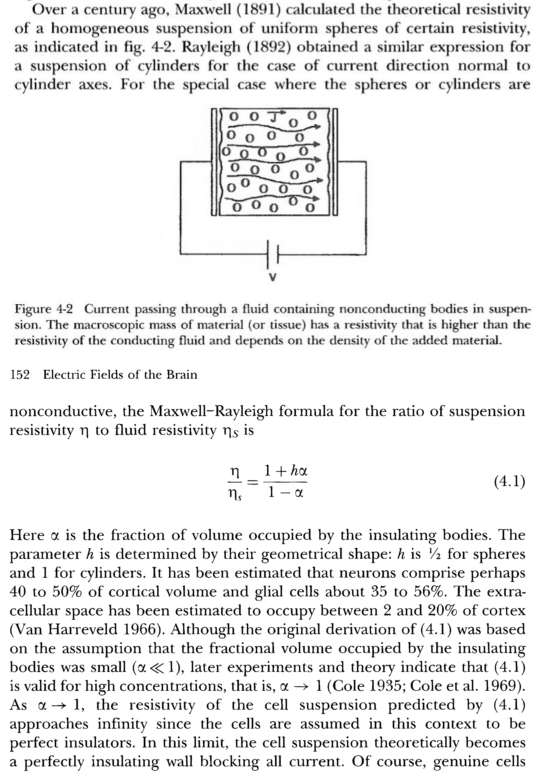
\includegraphics[width=0.6\textwidth]{Figures/Sigma/resistivity_maxwell.png}
%\end{center}
%\caption{\textbf{From Nunez} \tvnnote{Ta med noe slikt?}}
%\label{Sigma:fig:maxwell_resistivity}
%\end{figure}


%%%%%%%%%%%%%%%%%%%%%%%%%%%%%%%%
\section{\blue{Anisotropic conductivity}}
\label{sec:Sigma:Anisotropic}
\index{Conductivity!Anisotropic}
%%%%%%%%%%%%%%%%%%%%%%%%%%%%%%%%
In \fref{chap:VC}, we assumed that the tissue conductivity ($\sigma_\text{t}$) was isotropic, 
i.e., the same in all the spatial directions. 
However, the tissue of many brain regions have clearly anisotropic geometrical properties, 
and it is reasonable to assume that such anisotropy should be reflected in the conductivity. 
For example, cortex is to a large degree populated with pyramidal neurons that tend to be
geometrically aligned along the depth direction of cortex, and indeed, 
conductivity measurements have found that $\sigma_\mathrm{t}$ is about 1.5 times larger in the depth direction
(parallel to the axis of pyramidal cell dendrites) than in the lateral direction \cite**{Goto2010}. 
The cerebellum has an even more pronounced anisotropic geometrical structure, 
and in the anuran cerebellum, $\sigma_\mathrm{t}$ has been found to be about 3 times larger 
in the depth direction than in the lateral direction \cite**{nicholson1975}. 
A pronounced anisotropy in the conductivity is typically observed in white matter, 
because the axons tend to be oriented in similar directions by the formation of fiber bundles \cite**{Nicholson1965,Logothetis2007,Bangera2010}. 
This anisotropy can in certain cases cause a 10-fold increase in conductivity along the fiber bundle \cite**{Nicholson1965,Bangera2010}.

The overall effect of the anisotropy on extracellular potentials, 
at least in cortex, often appears to be quite weak \cite**{Logothetis2007,Ness2015,Miceli2017}, 
and the approximation that $\sigma_\text{t}$ is isotropic often gives good predictions of the potential.
An example is given in \fref{fig:Sigma:anisotropy_effect}, where a 1.5-fold increase in the conductivity 
along the axis of the apical dendrite (as suggested by \cite**{Goto2010}), 
only causes a slightly more squeezed shape of the extracellular potential 
compared the isotropic case \cite**{Ness2015,Miceli2017}. 
Since extracellular potentials are rather insensitive to modest anisotropies, 
it is common to make the modeling approximation that  $\sigma_\text{t}$ is isotropic.

\begin{figure}[!ht]
\begin{center}
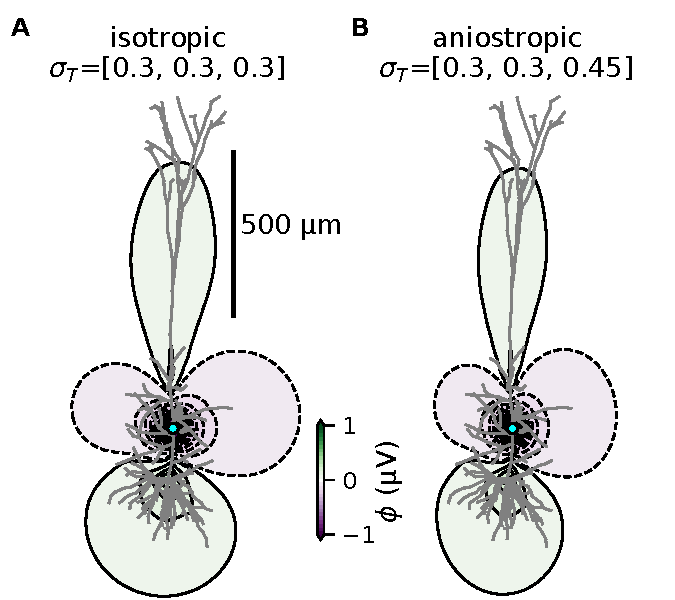
\includegraphics[width=0.6\textwidth]{Figures/Sigma/fig_anisotropy_effect.pdf}
\end{center}
\caption[]{\textbf{Effect of modest anisotropy.}
Extracellular potential following a single excitatory synaptic input (location marked by cyan dot) to a rat cortical layer 5 pyramidal neuron \cite**{Hay2011}. The extracellular potential is shown at the time when it was at its maximal value in the case of ({\bf A}) 
an isotropic extracellular medium, or ({\bf B}) an anisotropic extracellular medium with a 50\% higher
conductivity along the axis of the apical dendrite. The same neural simulation was used in ({\bf A}) and ({\bf B}). In ({\bf B}), the extracellular potential was calculated using \fref{eq:Sigma:Panisos}. \ghnote{Opprinnelig figurtekst framsto som litt rotete. Sjekk at det som staar er korrekt.}
}
\label{fig:Sigma:anisotropy_effect}
\end{figure}

%\tvnnote{Give example already here of where this is particularly relevant?: White matter, Cerebellum, and also mention 50\% increase in cortex, from Goto.}
When deemed necessary, 
it is relatively straightforward to expand the VC theory to the case of an anistotropic $\sigma_\text{t}$. 
Then,  $\sigma_\text{t}$ will no longer be a scalar, 
but instead a tensor with the three components $\sigma_{tx}$, $\sigma_{ty}$ and $\sigma_{tz}$. 
If we use the point-source approximation (\fref{eq:VC:pointsources}), 
the extracellular potential surrounding a set of point current sources $I_k$ is given by \cite**{nicholson1975,Parasnis1986}:

\begin{equation}
\phi(x,y,z) = \sum_k \frac{I_k}{4\pi\sqrt{\sigma_{ty}\sigma_{tz} (x-x_k)^2 + \sigma_{tx}\sigma_{tz} (y-y_k)^2 + \sigma_{tx}\sigma_{ty} (z-z_k)^2}}.
\label{eq:Sigma:Panisos}
\end{equation}
A derivation of this equation is found in \fref{app:Aniso}.

If we use the CSD-description of the sources (eq.~\ref{VC:eq:csds}), the corresponding expression is:
\begin{equation}
\phi(x,y,z) = \iiint_V \frac{C(x,y,z)}{4\pi\sqrt{\sigma_{ty}\sigma_{tz} (x-x_k)^2 + \sigma_{tx}\sigma_{tz} (y-y_k)^2 + \sigma_{tx}\sigma_{ty} (z-z_k)^2}} \, dV.
\label{eq:Sigma:Canisos}
\end{equation}


%\ghnote{Trenger vi en presisering her? Hva betyr det at effekten er lav? Jeg tenker at 50 prosent stoerre sigma burde gi 50 prosent stoerre amplituder, og det er vel ikke en svak effekt? Mener vi at spenningen i en utvalgt retning er relativt upaavirket av anisotropi i andre retninger enn den utvalgte?}
%\tvnnote{La til figur. Vi ble overasket i Ness et al. (2015), over at det nesten ikke var noe synlig effect, hverken naar det var simulert med FEM eller med punktkilde-formlene. Forskjellen kan kanskje kvantifiseres bedre, men er det noe vits?}


%%%%%%%%%%%%%%%%%%%%%%%%%%%%%%%%
\section{\blue{Inhomogeneous conductivity}}
\label{sec:Sigma:nonhomo}
\index{Conductivity!Inhomogeneous}
\tvnnote{In- or non-homogeneous?}
\ghnote{Begge deler brukes i litteraturen. Byttet til Inhomogeneous.}
In \fref{chap:VC}, we assumed that the extracellular conductivity $\sigma_\text{t}$ was homogeneous, 
i.e., the same everywhere. 
As we illustrated in \fref{fig:Sigma:ECS}, this assumption clearly does not hold on the micrometer scale, 
where neural tissue is highly inhomogeneous \cite**{Nicholson1998}.
Also, it clearly does not hold on the very large scale, since, 
if we travel far enough through brain tissue we will pass through boundaries between different tissue types 
with different conductivities. Eventually, we will also run into the less conducting skull.

%On a very large spatial scale, for example at the scale of whole brains, it is again clear that the tissue is non-homogeneous, since the brains, even for large primates, are not infinite in size.
However, on a mesoscopic spatial scale, the microscale inhomogeneities 
tend to average out (cf. the continuous medium approximation), 
and at the same time, the boundaries to other tissue types or materials are often sufficiently distant 
to have a negligible effect on local extracellular potentials. 
In such cases, for example within a given brain region such as cortex, 
a homogeneous conductivity appears to be a reasonable approximation \cite**{nicholson1975,Okada1994,Logothetis2007,Goto2010,Ness2015}.

There are however still many scenarios where an infinite homogeneous medium is not a reasonable assumption,
typically because of boundaries between neural tissue and other tissue types or materials.
%For example, for electric potentials measured close to the surface of the brain, the transition from neural tissue  (like for ECoG measurements, see also \ref{chap:ECoG}),
%The situation is different when signals are recorded very far from their sources. It is then likely that they on their journey have experienced a $\sigma_\text{t}$ that varied on a macroscopic scale \tvnnote{Er det egentlig riktig aa snakke om "reisen" til et potensial? }.
%For example, electroencephalography (EEG) signals recorded outside of the head are strongly affected by the presence of the brain tissue, cerebrospinal fluid (CSF), skull and scalp, which are very different media with different electrical  conductivities.
When the extracellular medium is inhomogeneous, there is no general analytical formula available 
(like eqs. \ref{VC:eq:csds}, \ref{eq:Sigma:Panisos} or \ref{eq:Sigma:Canisos}) 
that link the extracellular potentials to the underlying current sources. 
In principle, one can still always solve eq. \ref{VC:eq:CSD2} for arbitrarily complex geometries 
with varying conductivities using numerical methods, like the Finite Element Method (FEM) \cite**{Logg2012}. 
This approach has for example been used to model electroencephalography (EEG) signals 
recorded outside of the head, because these potentials are not only affected by the conductivity of brain tissue, 
but also by the presence of the cerebrospinal fluid (CSF), skull and scalp, which have widely different conductivities. 
\ghnote{Sitering paa dette?} EEG-modeling is covered in more detail in \fref{chap:EEG}. 
Substantial inhomogeneities can also be introduced into neural tissue through the presence of big electrode shanks, 
as briefly discussed in \fref{sec:VC:elec_shafts}.
%For examples of neuroscience applications using this approach, see \cite**{Moffitt2005,Frey2009,Joucla2012,Haufe2015,Ness2015,Buccino2019b,Obien2019}.


\subsection{\blue{Planar boundaries: The cortical surface and {\it in vitro} slice recordings}}
\ghtxt{\sout{
For some simple and highly symmetric cases of inhomogeneous volume conductors, 
analytical solutions can be found for extracellular potentials evoked by underlying current sources. 
For example,}}\ghnote{Her ble "planar boundaries" introdusert som et eksempel, men vi gir ingen andre eksempler.
Finnes de? Jeg tok bort den introen. Hvis det finnes andre eksempler, kan vi ta den tilbake, men da boer vi nevne dem.} 

As we explained above, analytical solutions for extracellular potentials in inhomogeneous
volume conductors can generally not be found. However, analytical solutions do exist
for idealized cases with planar boundaries between different tissue-types or different materials.
In such cases, the \textit{Method of Images} (MoI)\index{Method of Images} from electrostatics \cite**{Jackson1998} 
can be used to account for the effect of a planar boundary on the extracellular potential 
arising from underlying current sources \cite**{Gold2006,Pettersen2006,Nunez2006,Ness2015,Obien2019}. 
This method is based on introducing virtual current sources on the opposite side of the boundary 
with the same distance to the boundary as the original point current sources,
and with the amplitudes scaled by \cite**{Nunez2006,Ness2015},
\begin{equation}
W = \frac{\sigma_1 - \sigma_2}{\sigma_1 + \sigma_2}, 
\label{eq:Sigma:MoI_scaling}
\end{equation}
where $\sigma_1$ is the conductivity of the region containing the real current sources,
and $\sigma_2$ is the conductivity of the region on the other side of the boundary containing the virtual sources.

The MoI has been used to model effects near the cortical surface during {\it in vivo} recordings.
In such recordings, the cortical surface\index{Cortical surface! Measurement effects} must typically be exposed
before inserting recording electrodes into the brain,
and materials of widely different conductivity can be used to cover the cortical surface during the recordings. 
Using MoI, the different conductivity of cortex and the cover material
can be accounted for by modifying the point source equation (\ref{eq:VC:pointsource2})
to \cite**{Nicholson1971,Pettersen2006}:
\begin{equation}
\phi({\bf r}) = \frac{I_k}{4\pi \sigma_\text{t} |{\bf r-r_k}|} + \frac{\sigma_\text{t} - \sigma_{\rm cover}}{\sigma_\text{t} + \sigma_{\rm cover}} \frac{I_k}{4\pi \sigma_\text{t} |{\bf r-r_k'}|},
\label{eq:Sigma:MoI}
\end{equation}
where ${\bf r}_k'$ is the location of the virtual current source, mirrored across the cortical surface.
Note that this equation is only valid within the region with the real source, 
while other formulas apply outside of this region \cite**{Nunez2006}.

The material at the cortical surface can substantially affect potentials measured near the cortical surface, 
as illustrated in \fref{fig:Sigma:cortical_surface_effect}. 
In particular, notice from \fref{eq:Sigma:MoI} the special case of a measurement 
performed at the planar boundary to a non-conducting region, 
so that $|{\bf r-r_k}|=|{\bf r-r_k'}|$, and $\sigma_{\rm cover}=0$. 
In this case, the measured potential will be exactly a factor of two larger than for an infinite homogeneous medium.

\begin{figure}[!ht]
\begin{center}
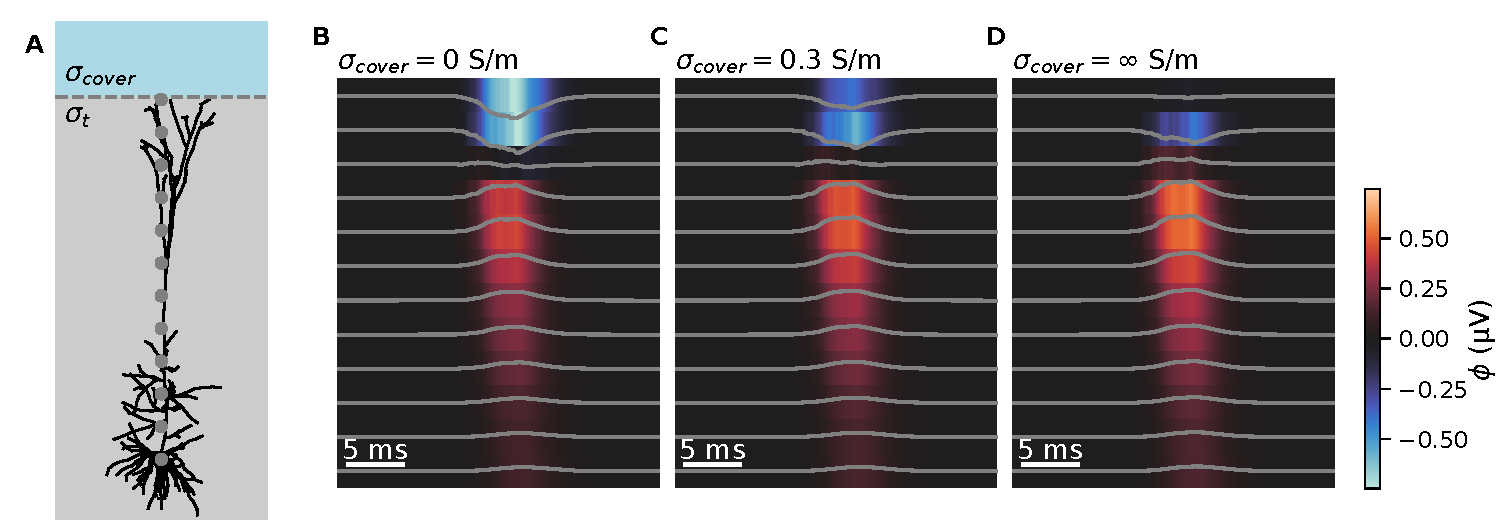
\includegraphics[width=1\textwidth]{Figures/Sigma/fig_cortical_surface_effect_MoI.pdf}
\end{center}
\caption[]{\textbf{Effect of inhomogeneity of cortical surface}
{\bf A:} Simulation set-up. A rat cortical layer 5 pyramidal cell \cite**{Hay2011} 
receives a wave of excitatory synaptic input to the upper apical dendrite (top 200~$\mu$m). 
The conductivity of cortical tissue is $\sigma_\text{t}$=0.3~S/m, 
while different conductivities of the region above cortex is tested.
{\bf B:} The cover is an insulator, $\sigma_{\rm cover}$ = 0.0~S/m, like a non-conducting mineral oil or air.
{\bf C:} The cover has the same conductivity as tissue, $\sigma_{\rm cover}$ = 0.3~S/m, 
corresponding to an infinite homogeneous volume conductor.
{\bf D:} The cover is highly conductive, $\sigma_{\rm cover}$ = $\infty$~S/m, like a metal plate.
See also \citeasnoun**{Pettersen2006}.
}
\label{fig:Sigma:cortical_surface_effect}
\end{figure}
%%%%%%%%%%%%%%%%%%%%%%%%%%%%%%%%

The MoI framework can also be used to model {\it in vitro} slice recordings\index{Slice recordings}, 
where a small slice of neural tissue is extracted from a brain and placed on a micro-electrode array (MEA), 
immersed in a saline bath. In this case, there are two planar boundaries:
the lower boundary between the slice and the non-conducting MEA (glass) electrode plate, 
and the upper boundary between the slice and the saline bath (\fref{fig:Sigma:MEA_illustration}).
Having two boundaries instead of one gives rise to an infinite series of virtual current sources (mirrors of mirrors),
which for the simplest case of the measurement being performed at the lower boundary 
to a non-conducting region, can be written like:
\begin{eqnarray}
\label{eq:Sigma:moi_PS}
\phi(x,y,0) & =  & \frac{2I}{4\pi \sigma_\text{t}} \bigg( \psi_{PS}(x,y,z')  \nonumber \\
& + & \sum_{n=1}^{\infty} W_{TS}^n\bigg[ \psi_{PS}(x,y,-z' + 2nh) + \psi_{PS}(x,y,-z' - 2nh) \bigg ]\bigg),
\end{eqnarray}
with 
\begin{equation}
\psi_{PS}(x,y,\tilde z) \equiv \left((x-x')^2 + (y-y')^2 + \tilde z^2)\right)^{-1/2}.
\end{equation}
For further details, see \citeasnoun**{Ness2015}.

In the chapter about extracellular spikes (\fref{fig:Spikes:MEA-spikes}), we show an example using the MoI framework
to model spikes in {\it in vitro} slices. 

\begin{figure}[!ht]
\begin{center}
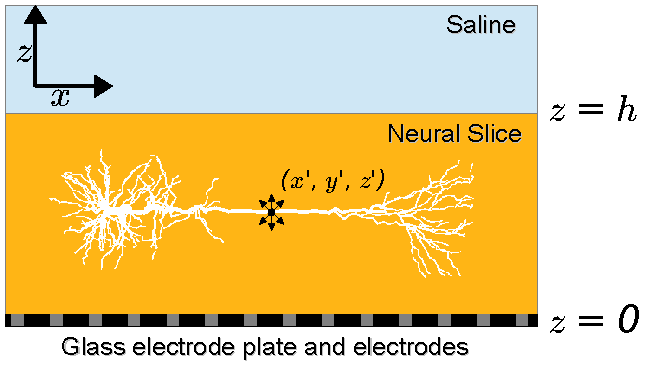
\includegraphics[width=0.4\textwidth]{Figures/Sigma/MEA_illustration.pdf}
\end{center}
\caption[]{\textbf{Illustration of MEA recording set-up.}
See also \citeasnoun**{Ness2015}.
}
\label{fig:Sigma:MEA_illustration}
\end{figure}
%%%%%%%%%%%%%%%%%%%%%%%%%%%%%%%%


